\chapter{Anwendung}\label{ch:anwendung}

Um mithilfe der Playbooks aus diesem Projekt einen Kubernetes-Cluster einzurichten, müssen zunächst die WiFi-Infrastruktur und die Raspberry Pis vorbereitet werden.
Dazu werden die SD-Karten einzeln mit Raspbian beschrieben und mit dem Playbook \texttt{local-""raspbian.yaml} für den Headless-Betrieb\footnote{Betrieb ohne Bildschirm} konfiguriert, mit Strom versorgt und gestartet.
Sobald alle Raspberry Pis online sind, wird Kubernetes mit dem Playbook \texttt{kubernetes.yaml} aufgesetzt.

\begin{figure}[h]
    % https://www.draw.io/?title=ansible-kubernetes-anwendung#R7Vlbd6IwEP41PuoBgoqPK73stt2trdt2%2B7QnSoTUQNgQqu6v3wBBwFhLd721Z33wkEkml2%2Fmm5lAA9j%2B%2FJzB0PtKHUQahubMG%2BCkYRidblf8J4JFJgAdLRO4DDuZSC8EQ%2FwbSWE%2BLMYOiioDOaWE47AqHNMgQGNekUHG6Kw6bEJJddUQukgRDMeQqNIH7HAvk1pGt5B%2FRtj18pX1Ti%2Fr8WE%2BWJ4k8qBDZyUROG0Am1HKsyd%2FbiOSYJfj8vBl8UCupp3zi5voF7zrX37%2Fdt%2FMJjt7i8ryCAwF%2FK%2Bnvn6M4N2nm%2Blvt%2Bs%2F65bZu7%2F50ZRnfYYklnjJs%2FJFDiByBJ6ySRn3qEsDSE4LaZ%2FROHBQsowmWsWYK0pDIdSF8AlxvpDOAWNOhcjjPpG9Nc8ncYhozMZow6GAdDPIXMQ3jLOycckBS74i0TtH1EecLcQAhgjk%2BLnqUFD6pbscV2AvHiT8bzAFUExxC6NwhGGQaAYRh4RgJCBSLFTgn4A58zBHwxCmEM0Ep%2F8F62fEOJpvRCfvNSVNZJzoyeasIJ2exwSvRLhcbft4gkO4Mppj%2FiNRb7Vl67HUczKXM6eNRd4IxHlLSknzsdxXqKWtXG%2FLtLFq0gYYR8UbS%2BHNgMDFiNJpw%2BgQcZD%2BiIknl6eIZZIJFYiJZAIlIJ1fcRLF%2B7bASHBMdH1Ds0KcqxMq8kqTLWmZTSZ2nc1XXaNYFcbRpGGDRt%2F23g199XZN%2FrZ3xV%2B995%2B%2Fb%2BKvXjfvgaPir64mvuFJ8xIKz00Tn%2Fi7wkE8bw7sZNM4IMh9LywCe0yC5On69IthfO1fxfZZ%2FMSjW%2FehaX7I%2Bs5QHX18ez%2B%2BnNoXZ5%2FC7sQ2m2LvI1kQH4uj59ve4OhpxYdYuqkBfnfuvrwqHSxpgI6CcYCwCt8%2BM0kpjxRZ5ZVMolfySJFW9pNJgFkzk%2BjHlUqAWgs%2BwUPaXv8b22vvw%2Fage1y2V1PdEAdOshQhKI2nUfI6ComLtIhv4mRnalD1qD%2BKo9cDKiTYDcTzWGAurgu7i7BAWynLawZYa1cFhZrDPkJBsXVXlqoDitOLprRm29JamviZJjBBx8qj5yJPii3NsNpd3cz%2BV6bPCClnXLHicov%2FwJ%2BuYtmd3aOnsShyAsRR9KHu0GZ7pRxq768aWktWXTHp8ZP1ADXHerLqRtWaq1bKoso2%2BLjWduqt%2BPhtVw60my5kr9cW5qFqi03bXn01X76oZVXFkQam1SqidmTaxnuJIbsdoMueb7oXJ95dYI1Ddr0GUdW7CcFhhKoIRR4Mk34UOEMOedI7wYTYlFCWqgEt%2FSVDOaNTtK7nBfjqIv8izG1r5e2PijJYAzLYFcg1wn8GUv5h1FgPtj93k0%2FDrQmhs7En%2FLyVevtP4wWP3hW%2BvX3BK5rFZ90soBffxsHpHw%3D%3D
    \centering
    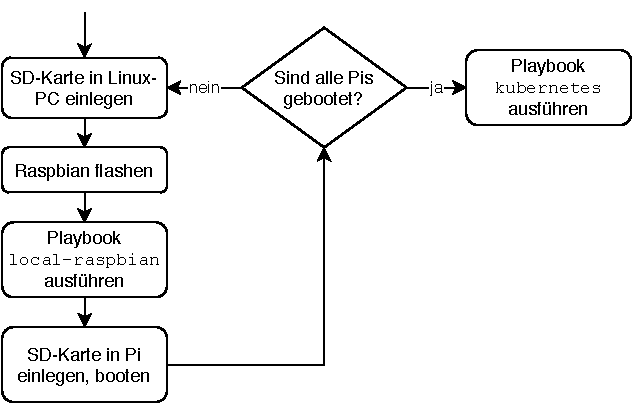
\includegraphics[width=.7\textwidth]{img/anwendung.pdf}
    \caption{Ablaufdiagramm zur Einrichtung eines Clusters}
\end{figure}

\section{Vorbereitung}\label{sec:vorbereitung}
Zum erfolgreichen Ausführen dieser Anleitung müssen folgende Voraussetzungen erfüllt sein:

\textbf{Raspberry Pis} in beliebiger Anzahl und ebenso viele Speicherkarten und Netzteile stehen bereit.

\textbf{Ein Linux-Rechner} steht bereit, um die Speicherkarten zu beschreiben und die Ansible-Playbooks auszuführen. Dafür sind Balena Etcher\footnote{\url{https://www.balena.io/etcher/} -- \today} und Ansible\footnote{\url{https://www.ansible.com/} -- \today} installiert, das Git-Repository zu diesem Projekt mit den Verzeichnissen \texttt{inventory} und \texttt{playbook} ist lokal verfügbar, außerdem ist ein Image von Raspbian Lite\footnote{\url{https://downloads.raspberrypi.org} -- \today} heruntergeladen.
% https://downloads.raspberrypi.org/raspbian_lite/images/raspbian_lite-2020-02-14/2020-02-13-raspbian-buster-lite.zip

\textbf{Ein Terminal} mit \texttt{playbook} als Arbeitsverzeichnis ist geöffnet.

\textbf{Ein WiFi-Access Point} mit Internetzugriff ist in Betrieb. Seine Einstellungen (IP, SSID, WPA2-Key) entsprechen den Angaben in den Dateien \texttt{inventory/""group\_vars/""all.yaml} und \texttt{playbook/""local-""raspbian.yaml}. Der zuvor erwähnte Linux-Rechner ist mit dem Access Point verbunden.

\textbf{Die Inventory-Datei} \texttt{inventory/""k8s-cluster.yaml} bildet den derzeitigen Cluster ab -- enthält also keine Einträge unter \texttt{hosts}, falls ein neuer Cluster eingerichtet werden soll:

\begin{lstlisting}[language=yaml, caption=Leere Inventory-Datei]
nodes:
  hosts:
\end{lstlisting}

\textbf{Ein SSH-Schlüsselpaar} ist generiert. Der private Schlüssel ist auf dem Linux-PC unter \texttt{\$HOME/"".ssh} hinterlegt und der öffentliche Schlüssel im Playbook \texttt{local-""raspbian"".yaml} in dem Array \texttt{sshKeys} angegeben.

\section{Raspbian installieren und Cluster einrichten}\label{sec:raspbian-installieren}
Die folgenden Schritte müssen für jeden Raspberry Pi einzeln durchgeführt werden.

\begin{enumerate}
    \item Speicherkarte in den Linux-Rechner einlegen.
    \item Raspbian-Image mit Balena Etcher auf der Speicherkarte installieren.
    \item Raspbian-Playbook ausführen:
        \begin{lstlisting}
sudo ansible-playbook -i ../inventory/k8s-cluster.yaml local-raspbian.yaml
\end{lstlisting}
    \item Speicherkarte in den Raspberry Pi einsetzen und starten.
\end{enumerate}

Wenn alle Raspberry Pis gestartet sind, wird die Installation mit dem Kubernetes-Playbook fortgesetzt:

\begin{lstlisting}
ansible-playbook -i ../inventory/k8s-cluster.yaml kubernetes.yaml
\end{lstlisting}

Der Kubernetes-Cluster ist anschließend einsatzbereit.

\section{Weitere Nodes hinzufügen}\label{sec:weitere-nodes-hinzufügen}

Sollen zu einem fertigen Cluster weitere Nodes hinzugefügt werden, kann auch dafür diese Anleitung ab Abschnitt~\ref{sec:vorbereitung} verwendet werden.
Die Inventory-Datei darf dann nicht leer sein, sondern muss die bereits vorhandenen Nodes enthalten.
